% main.tex, to be used with thesis.tex
% This contains the main work of your thesis.

%\bibliography{thesis}  % uses the references stored in Chapter1Radar.bib

\chapter{DSP Data Persistence: Component Design and Architecture}

In order to provide data to users, the RTC scientists use OPeNDAP \cite{opendap}
server to distribute collected data over the Internet. As discussed in the
previous chapter, this work proposes the use a Key-Value database system
in order to provide an alternative way for data persistence in sensor
networks, taking into account the taxonomies discussed earlier in chapter 
\ref{chap:taxonomies}. 

Considering our case study being NetBEAMS, and its infrastructure, this chapter
describes the design and architecture component designed specifically for the
Data Sensor Platform, DSP, in order to provide a persistence layer for
NetBEAMS. It is important to note that the technology chosen in the previous
chapter can be adapted by any alternative that uses the data model and
infrastructure options presented.

The proposed DSP Data Persistence component for the DSP Platform was
implemented by using the same approaches described in chapter
\ref{chap:netbeams-overview}. The following sections describe the scenarios
for persistence, analyzes the requirements from RTC, and describes the design
and architecture of the solution.

\section{Business Process Analysis}
\label{sec:business-process-analysis}
As described in section \ref{chap:netbeams-overview}, the DSP Platform was
designed to support an environmental sensor network based in San Francisco
Bay, composed by different types of sensors. The process of extracting the
measurements from the sensors to be reused through the DSP Platform can be
summarized following the UML Business Process Diagram \cite{uml} depicted in
figure \ref{fig:dsp-persistence-business-process}. It is important to note
that this diagrams details remote communication between sensor devices and a
centralized server, as part of the main scenario to solve the problem of data
persistence.

\begin{figure}[!b]
  \centering
  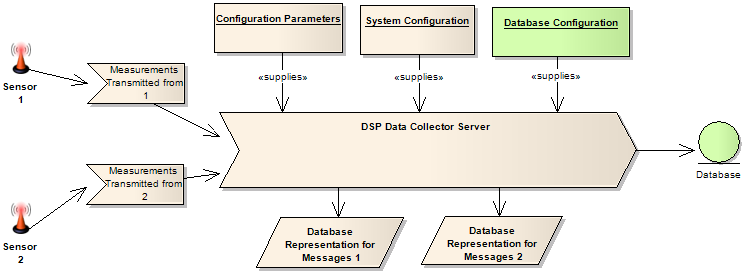
\includegraphics[scale=0.5]{../diagrams/DSP-DataPersistence-Business-Diagram}
  \caption{UML Business Process Model diagram - Adding Persistence for NetBEAMS}
  \label{fig:dsp-persistence-business-process}
\end{figure}

At the event of data collection, the DSP Client receives measurements collected
from each of the sensor devices. Each of the co-located DSP Client processes
the collected measurements and transforms them into the so-called DSP Message
(section \ref{sec:dsp-message}), which embodies the actual data values. After
proper data processing, transformation and categorization, the DSP Message is
added into temporary outbound queue. Then, as an asynchronous data
transmission event occurs with an specified rate, transferring all the queued
messages to be processed by a DSP Server host. As it is detailed in image
\ref{fig:dsp-persistence-business-process}, the server is centralized and is
able to concurrently process messages.

This work proposes the addition of a database system that is responsible for
storing the gathered measurement data from sensor nodes of the SF-BEAMS through
the use of NetBEAMS. Also in figure \ref{fig:dsp-persistence-business-process}, 
the processed measurement data from sensors 1 through N must be collected in
the same fashion and categorized as necessary. In this way, end users such as
Biologists and/or Programmers can access the collected measurements directly
from the Database. Furthermore, the same measurement data can be exported to
different formats as the users find necessary.

As a matter of fact, the data measurements collected from the sensor devices
are simple properties with keys and associated values as described in section
\ref{sec:sfbeams}, after data has been described. According to the descriptions
of the DSP Platform and the DSP Messages structure, the data is represented in
programming language formats such as Java \cite{java} or in a serialized
version in XML \cite{xml}. Similarly, the collected data contains measurements
that uniquely identifies them, together with other properties such as time
stamps of data creation and collected, as well as the the IP
address\footnote{Internet Protocol Address} of the DSP Client that produced
the data. Therefore, these are important properties for the proposed solution
of this work.

\section{Requirements Specification}

By analyzing the main scenario of collected data in the previous section, as
well as by collected requirements from the RTC staff, this section lists the
main use cases that the system and the primary users require. One of the
primary requirements of the system is to enable the use a persistence system
that does not promote the use of specialized professionals to deal with data
modeling, as it is required in most projects using the Structured Query
Language (SQL) \cite{sql}, used to extract data from a Relational Databases.

\subsection{Functional Requirements}
\label{sec:use-cases}

As part of the user stories related to data access, figure
\ref{fig:DSP-Data-Persistence-UseCases-Diagram-Users} describes the use cases
that the end users can perform with the system.

\begin{figure}[!b]
  \centering
  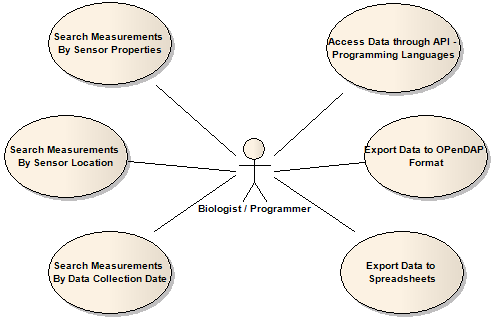
\includegraphics[scale=0.5]{../diagrams/DSP-Data-Persistence-UseCases-Diagram-Users}
  \caption{UML Use Case diagram for Persistence Functions}
  \label{fig:DSP-Data-Persistence-UseCases-Diagram-Users}
\end{figure}

The functional requirements listed in this section are in the format of UML
User Cases Diagrams \cite{uml}. Figure
\ref{fig:DSP-Data-Persistence-UseCases-Diagram-System} summarizes the use 
cases that the system, as the main actor of the system, must perform:

\begin{itemize}
  \item \textbf{Search Measurements by Sensor Properties}: users of the
  collected data must be able to search data through the properties of the
  sensors. This is related to identity principle of what was collected
  as provenance \cite{db-provenance};
  \item \textbf{Search Measurements by Sensor Location}: users of the collected
  data must be able to search data by a given sensor location, as referred to
  the provenance from where the data was collected;
  \item \textbf{Search Measurements by Data collection date}: users of the
  collected data must be able to search data by a given date, or ranges of
  start and end date;
  \item \textbf{Access the data through API, Programming Languages}: users of the
  collected data must be able to search data by the use of different
  programming and scripting languages of their preference;
  \item \textbf{Export Data to OPEnDAP format}: users of the collected data
  must be able to export the collected data to the OPEnDAP format;
  \item \textbf{Export Data to Spreadsheets}: users of the collected data must
  be able to export the collected data to spreadsheets.
\end{itemize}

\subsection{Non-Functional Requirements}

\begin{itemize}
  \item The DSP Data Persistence component must maintain the received DSP
  Measurement Messages in-memory for a specific rate in order to decrease the
  write load on the database;
  \item The Persistence storage system must be able to cope with dozens of DSP
  Messages;
  \item The Persistence storage system must be able to save measurements quickly;
  \item The Persistence storage system must be able to scale without too much
  architectural changes, or schema changes;
  \item The Persistence storage system must not impose the knowledge of
  complicated database system languages such as SQL \cite{sql} or XML XPath
  \cite{xml-xpath}, but use access through API calls, as it offers better
  abstractions for non-computer science researchers
  \cite{sn-programming-language}.
\end{itemize}

\section{Data Model Design}
\label{sec:dsp-persistence-data-model}

As described in the previous chapter, the data model that might give better
support for collected data from sensor networks is the Key-Value-Pair Data
Model. Beyond the data collected from the sensor devices, Data Provenance 
techniques must also be considered to better describe the collected data
\cite{sn-provenance}. In general, the data model must include the following
metadata besed on Data Provenance:

\begin{itemize}
  \item \textbf{Locality}: properties that describe the location of the data.
  For example, the host machine name or IP address, the GPS coordinate
  \cite{gps};
  \item \textbf{Identity}: what uniquely identities the data among the others
  produced by other sensor devices in the network, as for instance a
  UUID\footnote{Universally Unique Identifier};
  \item \textbf{Time-Dimensions}: when the data was ``sensed''
  \cite{db-provenance} and when the collection transaction happened
  \cite{sn-time-series}.
\end{itemize}

After analyzing the DSP Platform and the structure of the DSP Messages in
chapter \ref{netbeams-architecture}, the following set of keys are expected to
be part of the design of the data model. Any key represented by time or
location are related to the provenance support discussed in section
\ref{sec:sn-provenance}:

\begin{itemize}
  \item \textbf{sensor.ip\underline{ }address}: it is extracted
  from the DSP Message Produce and identifies which sensor generated the sampling;
  \item \textbf{sensor.location.latitude, longitude}: the latitude and
  longitude GPS coordinates of the position of the sensor device, captured from
  references of the device. This is currently provided as a parameter in the
  bootstrap message for the component;
  \item \textbf{message\underline{ }id}: it's extracted from each of the messages contained
  in the DSP Message Container;
  \item \textbf{time.transaction}: it is extracted from the DSP
  message container creation time and it is used to identify when the transaction occurred;
  \item \textbf{time.fact}: it is extracted from the
  SondeDataContainer's date and time, and identifies the time in which the
  collected data occurred.
\end{itemize}

It is important to note that this set of metadata must occur in every
collected data from any sensor device. However, on the contrary of the
metadata, a different set of properties will occur to describe the sensed
properties of a given sensor, and for this reason, the following structure is
defined to accommodate such data:

\begin{itemize}
  \item \textbf{observation}: this key defines the values of the document, and
  will have every different property of the sensor. For instance, the data key for the
  properties of the YSI device will contain the set of properties defined for
  the device, such as battery, temperature, salinity, etc.
\end{itemize}

\section{High-Level System Architecture}

Considering the business analysis described in section
\ref{sec:business-process-analysis}, the addition of a data persistence layer
to the DSP Platform can be achieved by adding Data Consumer (DC) as described
in section \ref{netbeams-architecture}. Based on the Requirements
specification described earlier, this component must be responsible for
providing the processing of the DSP Measure Messages, extracting the payload of
the body of the message and converting it to the data model defined in the
previous section. Finally, the data can be transmitted to the chosen database
system. Figure \ref{fig:NetBEAMS-Persistence-Server-Node-Components} provides
an architectural view of the DSP Server node with the loosely-coupled
components, highlighting the inclusion of the DSP Data Persistence.

\begin{figure}[!b]
  \centering
  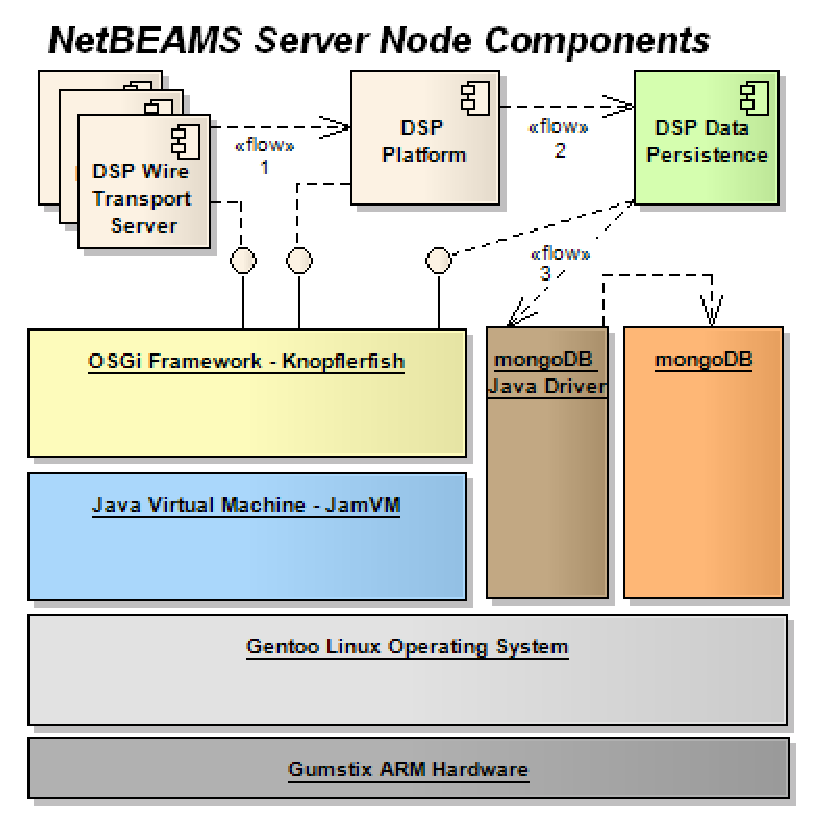
\includegraphics[scale=0.5]{../diagrams/NetBEAMS-Persistence-Server-Node-Components}
  \caption{UML Components diagram of the DSP Data Collector}
  \label{fig:NetBEAMS-Persistence-Server-Node-Components}
\end{figure}

As it is depicted in figure
\ref{fig:NetBEAMS-Persistence-Server-Node-Components}, the DSP Data
Persistence component can be added into the system as an independent
plug-and-play component. In addition, the database system and the necessary
drivers are also added without any changes to the existing DSP infrastructure.
First, as DSP Messages are delivered to the server through the DSP Wire
Transport Server, as shown by flow 1, the DSP Platform is responsible to
forward a copy of the Measurement messages directly to the DSP Data
Persistence as shown by flow 2. Then, the sole responsibility of the DSP Data
Persistence is to transfer the received measurement messages to the database
system by using the connection drivers, as depicted by flow 3.

The following sections focus on the DSP Data Persistence component design in
the context of an OSGi bundle \cite{osgi}.

\section{DSP Data Persistence: OSGi-DSP Bundle Design}

The new proposed Data Persistence component must follow the DSP requirements
for a new DSP Component, which specifies the design-pattern of Data
Producer/Consumer. In a nutshell, the design of a DSP Component maintains the
dependency among 3 different major Java packages: it depends on 2 existing
packages, namely the OSGi Framework and the DSP Platform, as well as and an
additional package for the database access driver API, as shown in the UML
Package Dependency Diagram \cite{uml} of Figure
\ref{fig:DSP-Data-Persistence-Packages-Dependency}.

\begin{figure}[!h]
  \centering
  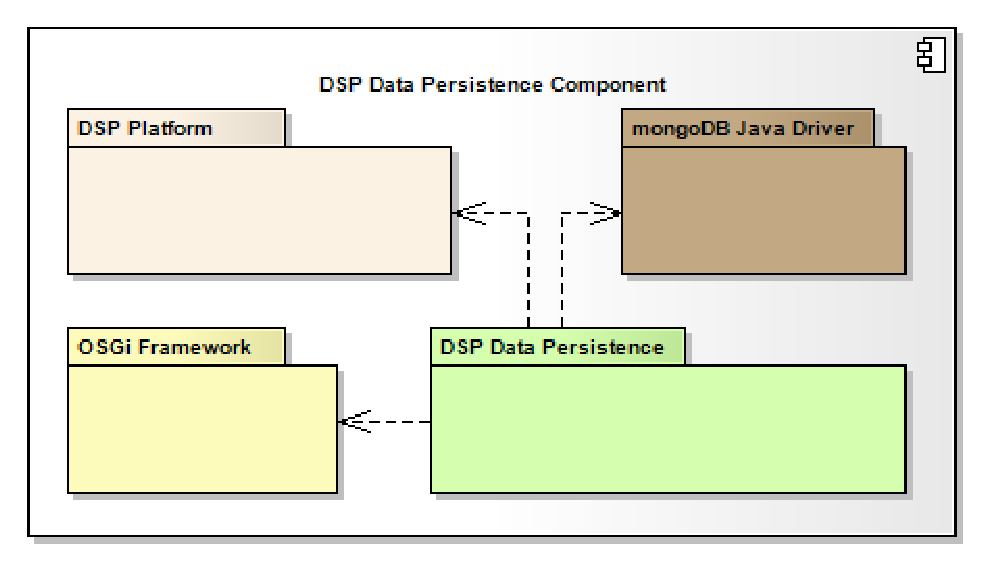
\includegraphics[scale=0.5]{../diagrams/DSP-Data-Persistence-Packages-Dependency}
  \caption{UML Components diagram of the DSP Data Collector}
  \label{fig:DSP-Data-Persistence-Packages-Dependency}
\end{figure}

The following sections details each step of the DSP Data Persistence activation
and parallel execution of the contained classes.

\subsection{DSP Data Persistence Activation and Message Delivery}

The DSP Data Persistence component starts with an OSGi Activator class, and the
implementation of the DSP Component, resposible to provide services to the
platform. Based on these specifications, the following set of classes in
figure \ref{fig:DSP-DataPersistence-Activator-Class-Diagram} shows the UML
Class Diagram \cite{uml} implemented for the component.

\begin{figure}[!h]
  \centering
  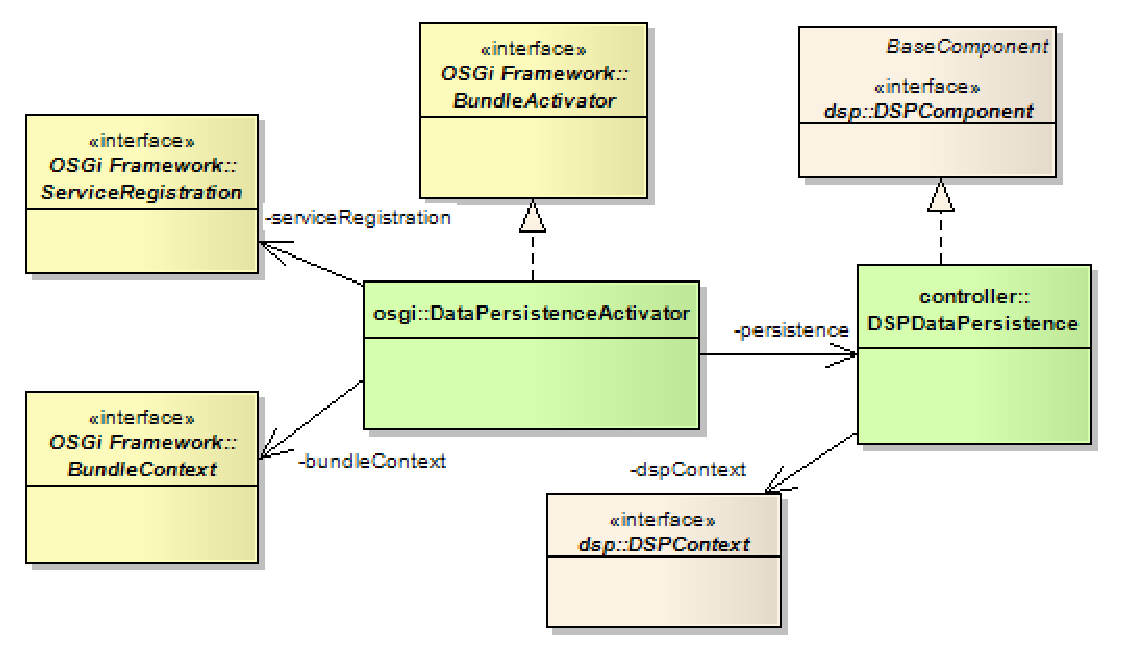
\includegraphics[scale=0.5]{../diagrams/DSP-DataPersistence-Activator-Class-Diagram}
  \caption{UML Class diagram for the DSP Data Persistence Activator and Component}
  \label{fig:DSP-DataPersistence-Activator-Class-Diagram}
\end{figure}

The DSP Data Persistence Activator is the main class responsible for the
activation of the DSP Data Persistence component, as it extends the OSGi class
BundleActivator and maintains a reference of the DSP Data Persistence class.
Furthermore, the activator maintains references to the classes BundleContext
and ServiceReference both from the OSGi Framework. The former is responsible
for maintaining the link with the OSGi Framework, while the latter is used to
register the DSP Component as a service. Therefore, it is clear that the class
DSP Data Persistence Activator is the main communication interface between the
DSP Platform and the OSGi Framework.

While the DSP Data Persistence Activator is responsible for the orchestration
of the classes during the execution on the OSGi Framework, the class DSP Data
Persistence extends from the DSP Platform class DSPComponent. For this reason,
this class inherits all the behavior described on \ref{netbeams-architecture}
and can be in the roles of Data Consumer and a Data Producer.

\begin{itemize}
  \item \textbf{DSP Data Persistence as Data Consumer}: receives any measurement
  message from remote sensors;
  \item \textbf{DSP Data Persistence as Data Producer}: transforms any
  measurement message received into a format that must be ready to be saved on the
  database, based on the description of the data model in section
  \ref{sec:dsp-persistence-data-model}.
\end{itemize}

The behavior of the activator class follows the specifications of the
OSGi Framework and, for this reason, instances of the DSP Data Persistence
Activator can be in the states described on the UML State Diagram depicted in
Figure \ref{fig:DSPPlatform-Install-Usage-State-Diagram}. It is important to
note that the activator is an extension of the OSGI class BundleActivator, as
well as being responsible for stopping or starting the the DSP Data Persistence
component instance. In this way, following the specifications of section
\ref{netbeams-architecture}, the DSP Data Persistence Platform can be
initialized as described as it is described by the UML Sequence Diagram of
Figure
\ref{fig:From-OSGi-Framework-to-DSP-Data-PersistenceActivator-Sequence-Diagram}:

\begin{enumerate}
  \item During the DSP Platform activation, it will get the name of the
  persistence component from the configuration artifact config.xml as seen in
  listing \ref{file:dsp-config.xml};
  \item After being selected based on the configuration priority, the DSP
  Bundle artifact is identified and installed, by creating an instance of the
  class DSP DataPersistence Activator and making a call to the method start();
  \item During the activation, an instance of the DSP Data Persistence
  component is created and registered as an OSGi Service;
  \item Upon registering the DSP Data Persistence component, the DSP Platform
  "listens" the event serviceUpdate() and, and triggers the last operations to
  bootstrap the DSP Component:
   \begin{enumerate}
      \item Initializes the component by calling the method initComponent();
      \item Starts the component by calling the method startComponent();
      \item Bootstrap messages are delivered to the component.
   \end{enumerate}
\end{enumerate}

Any configuration parameter required by a DSP Component is sent during its
bootstrap process through the use of an optional DSP Update Message, as shown
in Listing \ref{file:dsp-data-persistence-bootstrap.xml}. The initialization of
the DSP Component Activator and the DSP Component registration are also shown
in figure \ref{fig:From-OSGi-Framework-to-DSP-Data-PersistenceActivator-Sequence-Diagram}.

\begin{figure}[!b]
  \centering
  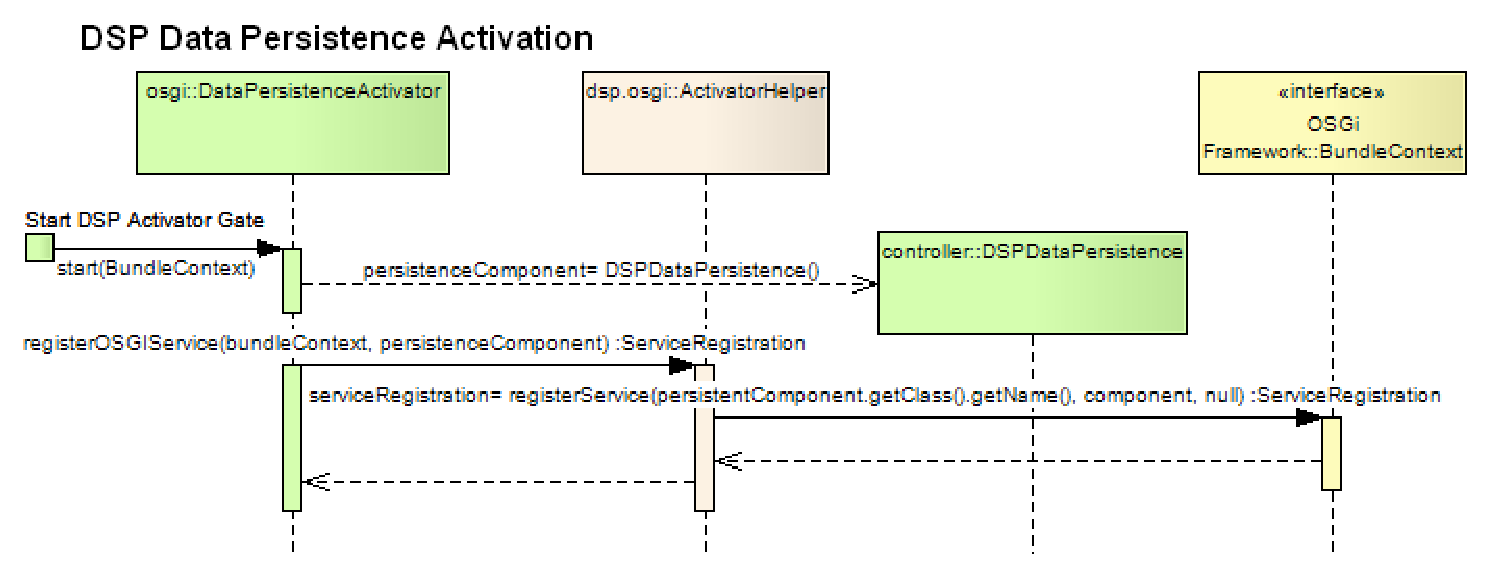
\includegraphics[scale=0.5]{../diagrams/From-OSGi-Framework-to-DSP-Data-PersistenceActivator-Sequence-Diagram}
  \caption{UML Sequence diagram describing the DSP Data Persistence bundle activation}
  \label{fig:From-OSGi-Framework-to-DSP-Data-PersistenceActivator-Sequence-Diagram}
\end{figure}

As soon as the gate "Start DSP Activator Gate" reaches the DSP Data
Persistence instance, it first creates the unique instance of the class DSP
Data Persisence and uses that instance to register it as the OSGi service
through the call to the DSP Platform helper class ActivatorHelper. At this
point, the DSP Data Persistence has been installed and is in the state
"Active".

\subsection{Delivering Bootstrap and Measurement Messages}

Although the DSP Data Persistence component has been instantiated as of image
\ref{fig:From-OSGi-Framework-to-DSP-Data-PersistenceActivator-Sequence-Diagram}, 
the process of delivering messages to the DSP Data Persistence has yet to be
completed. As defined by the requirements, the DSP Component must execute its
function in a concurrent fashion, using configuration parameters during its
bootstrap process. The class DSP Data Flusher is responsible for running as a
"worker thread", whose function is to verify if there are messages to be
flushed into the Database with the class Transient Persistence Layer. Figure 
\ref{fig:DSP-DataPersistence-Flusher-Classes} describes the UML Class
Diagram \cite{uml} for the main classes of this functionality.

\begin{figure}[!b]
  \centering
  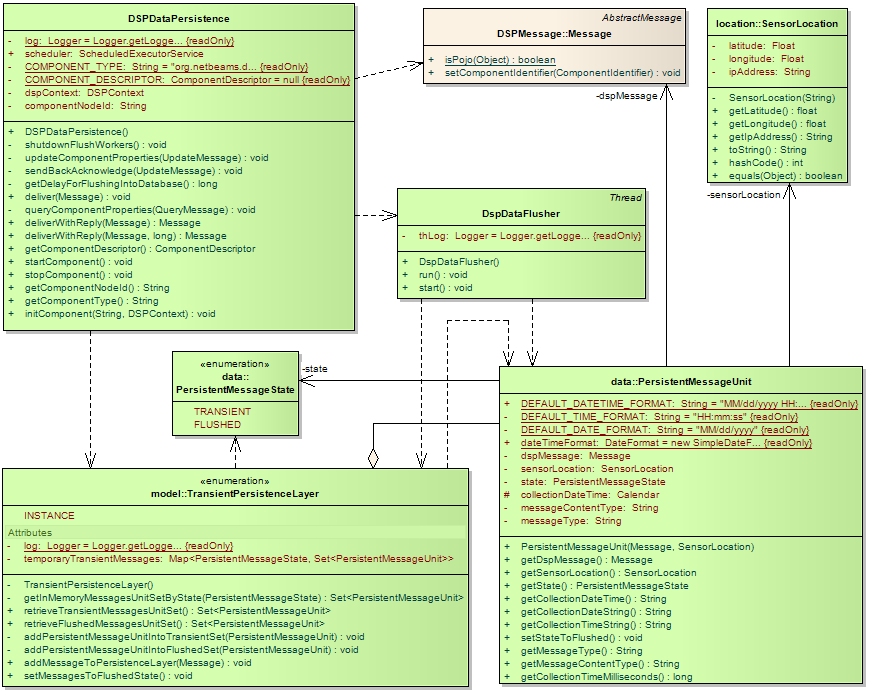
\includegraphics[scale=0.5]{../diagrams/DSP-DataPersistence-Flusher-Classes}
  \caption{UML Class diagram with the DSP Data Flusher worker thread}
  \label{fig:DSP-DataPersistence-Flusher-Classes}
\end{figure}

\begin{figure}[!b]
  \centering
  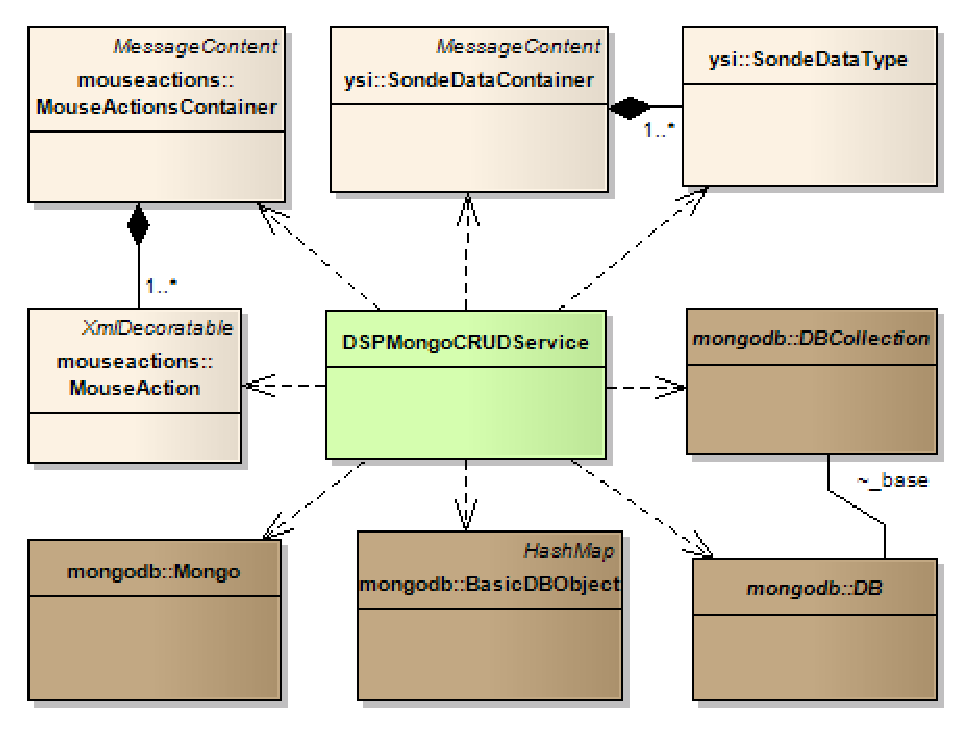
\includegraphics[scale=0.5]{../diagrams/DSP-Data-Persistence-Mongo-Classes}
  \caption{UML Class diagram with Persistence Service for MongoDB}
  \label{fig:DSP-Data-Persistence-Mongo-Classes}
\end{figure}

The DSP Data Flusher is a thread that is designed to be in two different
states as depicted in figure
\ref{fig:DSP-DataPersistence-Flusher-State-Diagram}: RUNNABLE and
TIMED\underline{ }WAITING. In the former state, the DSP Data Flusher will be
contacting the Transient Persistence Layer in order to verify if there are any
message in the outbound queue ready to be transmitted sent to the Database
service, while the DSP Data flusher will be waiting for the next cycle defined
by the bootstrap parameter TRANSIENT\underline{ }DATA\underline{
}FLUSHER\underline{ }DELAY in the latter state.

\begin{figure}[!b]
  \centering
  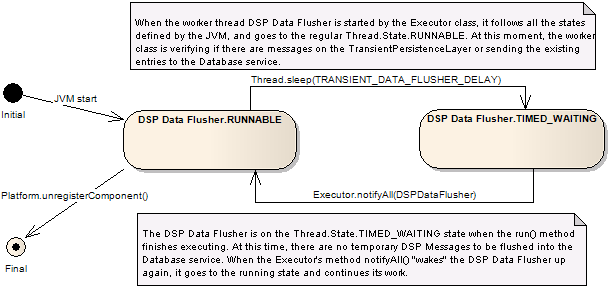
\includegraphics[scale=0.5]{../diagrams/DSP-DataPersistence-Flusher-State-Diagram}
  \caption{UML State diagram for the DSP Data Flusher Worker Thread}
  \label{fig:DSP-DataPersistence-Flusher-State-Diagram}
\end{figure}

Upon receiving a new DSP measurement message, the DSP Data Persistence
component must send its reference to the temporary memory space, as described
by the non-functional requirement in the beginning of this chapter. In this
way, the DSP Data Persistence component maintains a dependency on the Singleton
class TransientPersistenceLayer, which is responsible for keeping track of
messages that are received by working component. However, in order to add the
DSP message into its aggregated map, it first transforms the message into an
instance of the class PersistentMessageUnit, which has references to the class
regarding the location of the message, SensorLocation.

As depicted by the the UML Sequence Diagram \cite{uml} of figure
\ref{fig:From-DSPWireTransport-Server-To-DSP-Broker}, a DSP Message
is delivery to the DSP Broker for its delivery to Data Consumers configured to
receive that specific message. For this reason, Figure
\ref{fig:From-DSP-Broker-To-DSPDataPersistence-General-Sequence} continues the
steps of the DSP Broker from the gate "From DSP WireTransport Server to Broker
Gate", showing the steps taken to transfer a DSP Message to the Singleton
class TransientPersistenceLayer, responsible for maintaining a queue of
messages waiting to be sent to the database system.

According to the DSP Broker model described in section \ref{sec:dsp-message}, 
the DSP Matcher needs to be updated with the addition of a matching rule that
filters a copy of any Measurement Message to the DSP Data Persistence component
designed. As it is shown in figure
\ref{fig:From-DSP-Broker-To-DSPDataPersistence-General-Sequence}, the worker
Thread DSP Data Flusher is the link between the Transient and Persistent
layers, as it depends on the references from the classes
TransientPersistenceLayer and the DSPMongoCRUDService. The former maintains
DSP Messages in memory wrapped by an instance of PersistenceMessageUnit and
the latter is responsible for sending the MessageContent from the DSPMessage
body to the Database.

\begin{figure}[!b]
  \centering
  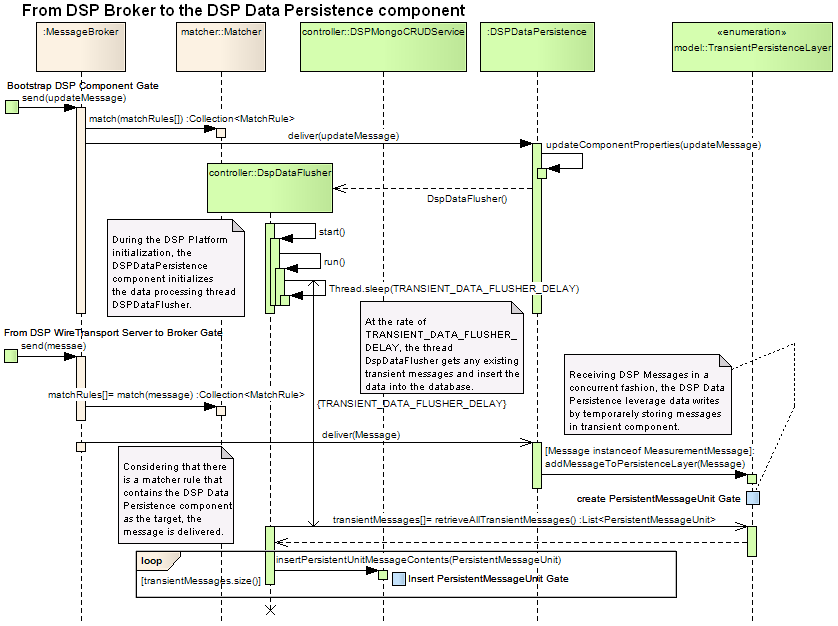
\includegraphics[scale=0.5]{../diagrams/From-DSP-Broker-To-DSPDataPersistence-General-Sequence}
  \caption{UML Sequence Diagram - Flow 1: From the DSP Broker to the Data
  Persistence Component}
  \label{fig:From-DSP-Broker-To-DSPDataPersistence-General-Sequence}
\end{figure}

The DSP Broker retrieves the list of matching rules by contacting the Matcher.
As the DSP Platform have already loaded all the Matching rules, a copy of a
given DSP message is delivered to the DSP Data Persistence component. However,
the sequence diagram shows two different stages of reception:

\begin{itemize}
  \item A bootstrap DSP Update Message is delivered to the DSP Data Persistence
  component when the DSP Platform is initializing the component. In this way,
  the DSP Data Persistence can initialize the DspDataFlusher worker thread to
  flush temporary messages into the database at the rate of
  TRANSIENT\underline{ }DATA\underline{ }FLUSHER\underline{ }DELAY in seconds,
  among others. Listing \ref{file:dsp-data-persistence-bootstrap.xml} shows an
  implementation of a bootstrap message for the DSP Data Persistence;
  \item Any DSP Measure Message can be persisted by the DSP Data Persistence
  component. When the DSP Broker delivers a DSP MeasureMessage to this
  component, it will add the message to a temporary memory location to decrease
  I/O on the database, as depicted by the gate "create PersistentMessageUnit
  Gate". This last gate describes the simple procedure to add the message
  into the transient persistent layer. Listing
  \ref{file:dsp-message-serialized-ysi}.
\end{itemize}

The class PersistenceMessageUnit is the major transient persistence unit that
carries references regarding the originating DSP Message that was collected by
the DSP Data Persistence component. It is composed by a SensorLocation and
contains a reference to the PersistentMessageState enumaration. The former
identifies which sensor produced the collected data from the DSP Message by the
IP address, while the latter identifies whether the PersistenceMessageUnit has
been saved into the Database or not as depicted by the UML State Diagram
\cite{uml} in Figure \ref{fig:PersistentMessageState-Diagram}.

\begin{figure}[!b]
  \centering
  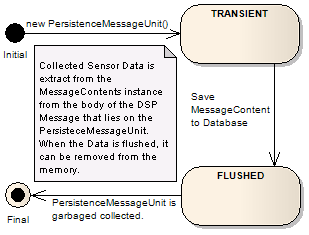
\includegraphics[scale=0.5]{../diagrams/PersistentMessageState-Diagram}
  \caption{UML State Diagram for the instance of the class
  PersistentMessageState}
  \label{fig:PersistentMessageState-Diagram}
\end{figure}

\begin{figure}[!b]
  \centering
  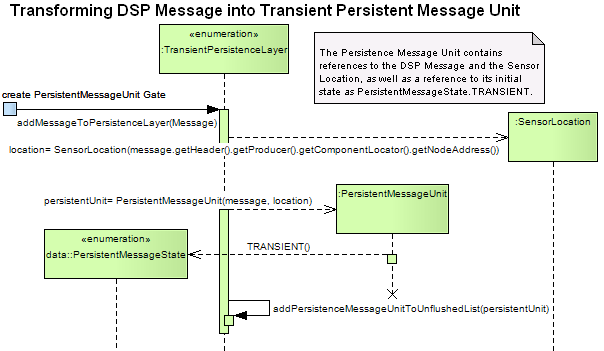
\includegraphics[scale=0.5]{../diagrams/From-Create-PersistentMessageUnit-to-TransientPersistence-Layer-Sequence}
  \caption{UML Sequence diagram - Adding a DSP Message into the Transient Persistence layer}
  \label{fig:From-Create-PersistentMessageUnit-to-TransientPersistence-Layer-Sequence}
\end{figure}

According to the data model specifications defined in section
\ref{sec:dsp-persistence-data-model}, the persistence model must carry
information regarding which sensor device produced the collected data. For
this reason, an instance of the class SensorLocation carries the information
about the IP address and and optional GPS location from the component that
originally produced the DSP Message. Then, an instance of the class
PersistenceMessageUnit is created at the state ``TRANSIENT'', as detailed
on UML State Diagram \cite{uml} in Figure \ref{fig:PersistentMessageState-Diagram}.

\subsection{Flushing data into the Database}

The last stage sequence described in the UML Sequence diagram of figure
\ref{fig:From-DSP-Broker-To-DSPDataPersistence-General-Sequence} depicts the
DspDataFlusher worker thread continuously waking up at the rate of
TRANSIENT\underline{ }DATA\underline{ }FLUSHER\underline{ }DELAY. Its purpose
is as simple as to iterate over the list of PersitenceMessageUnit on the state
of TRANSIENT, and send each of them to be saved on the persistence storage.
Figure \ref{fig:DSP-Data-Persistence-Classes} shows the participating classes
of the component.

\begin{figure}[!b]
  \centering
  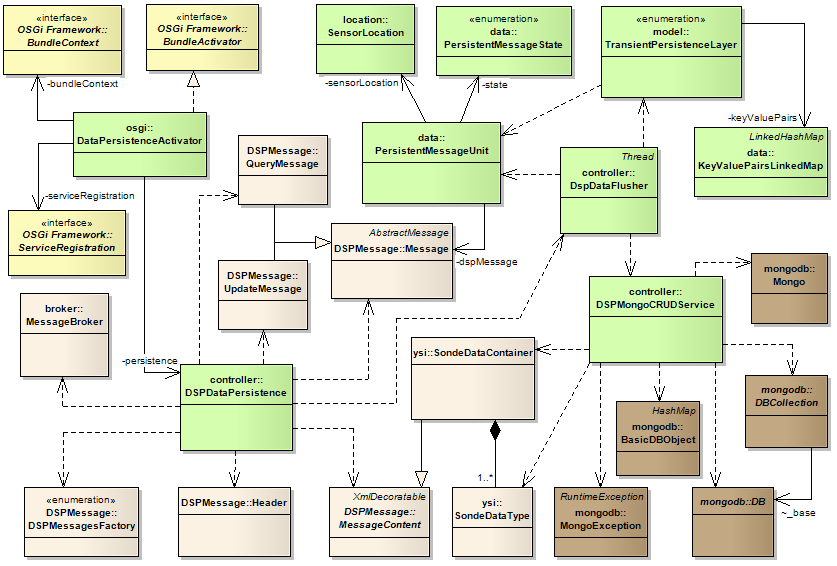
\includegraphics[scale=0.5]{../diagrams/DSP-Data-Persistence-Classes}
  \caption{UML Class diagram for the DSP Data Persistence component.}
  \label{fig:DSP-Data-Persistence-Classes}
\end{figure}

Finally, this sequence of events is continued by the "insert
PersistenceMessageUnit Gate", which triggers the persistence service from the
chosen database system as shown in figure
\ref{fig:From-Insert-PersistentMessageUnit-to-mongoDB}.

\begin{figure}[!b]
  \centering
  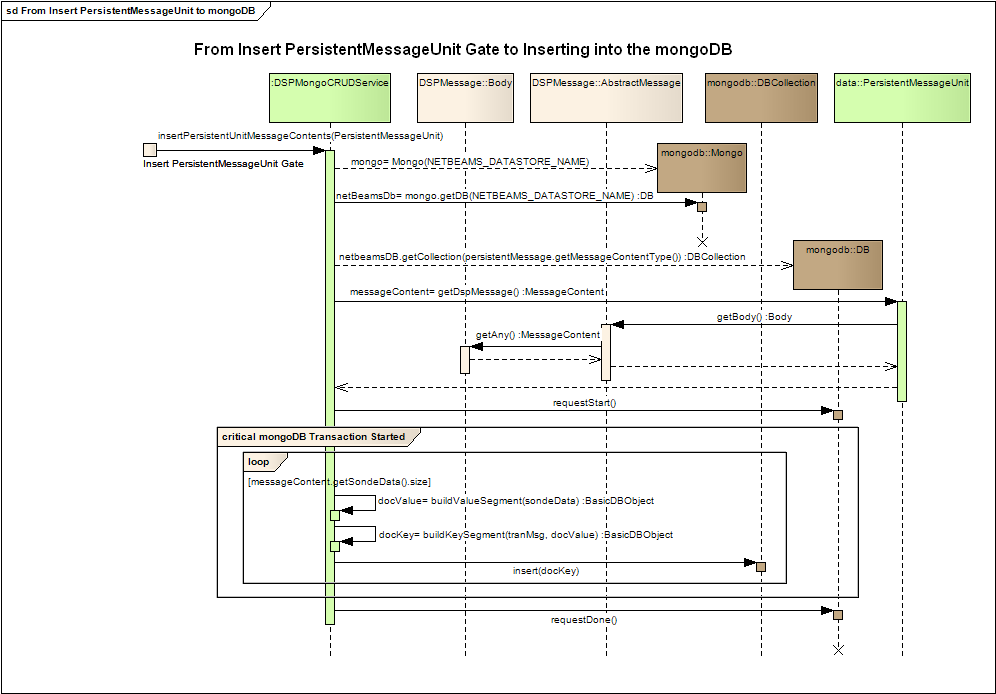
\includegraphics[scale=0.5]{../diagrams/From-Insert-PersistentMessageUnit-to-mongoDB}
  \caption{UML Sequence Diagram - MessageContent instance saved by the class
  mongoDB service}
  \label{fig:From-Insert-PersistentMessageUnit-to-mongoDB}
\end{figure}

In order to build the document key and value segments as described on section
\ref{sec:dsp-persistence-data-model}. First, the value is built by extracting
the DSP Message Content from the body of the DSP Message.

\begin{figure}[!b]
  \centering
  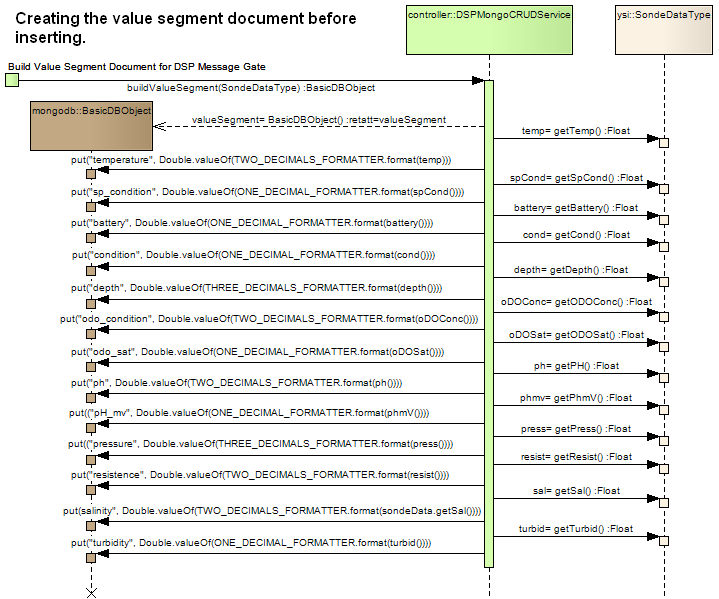
\includegraphics[scale=0.5]{../diagrams/From-Creating-Value-Segment-Sequence}
  \caption{UML Sequence diagram showing the creation of the value document segment}
  \label{fig:From-Creating-Value-Segment-Sequence}
\end{figure}

Finally, the document key segment is prepared as follows in figure
\ref{fig:From-Creating-Key-Segment-Sequence}.

\begin{figure}[!b]
  \centering
  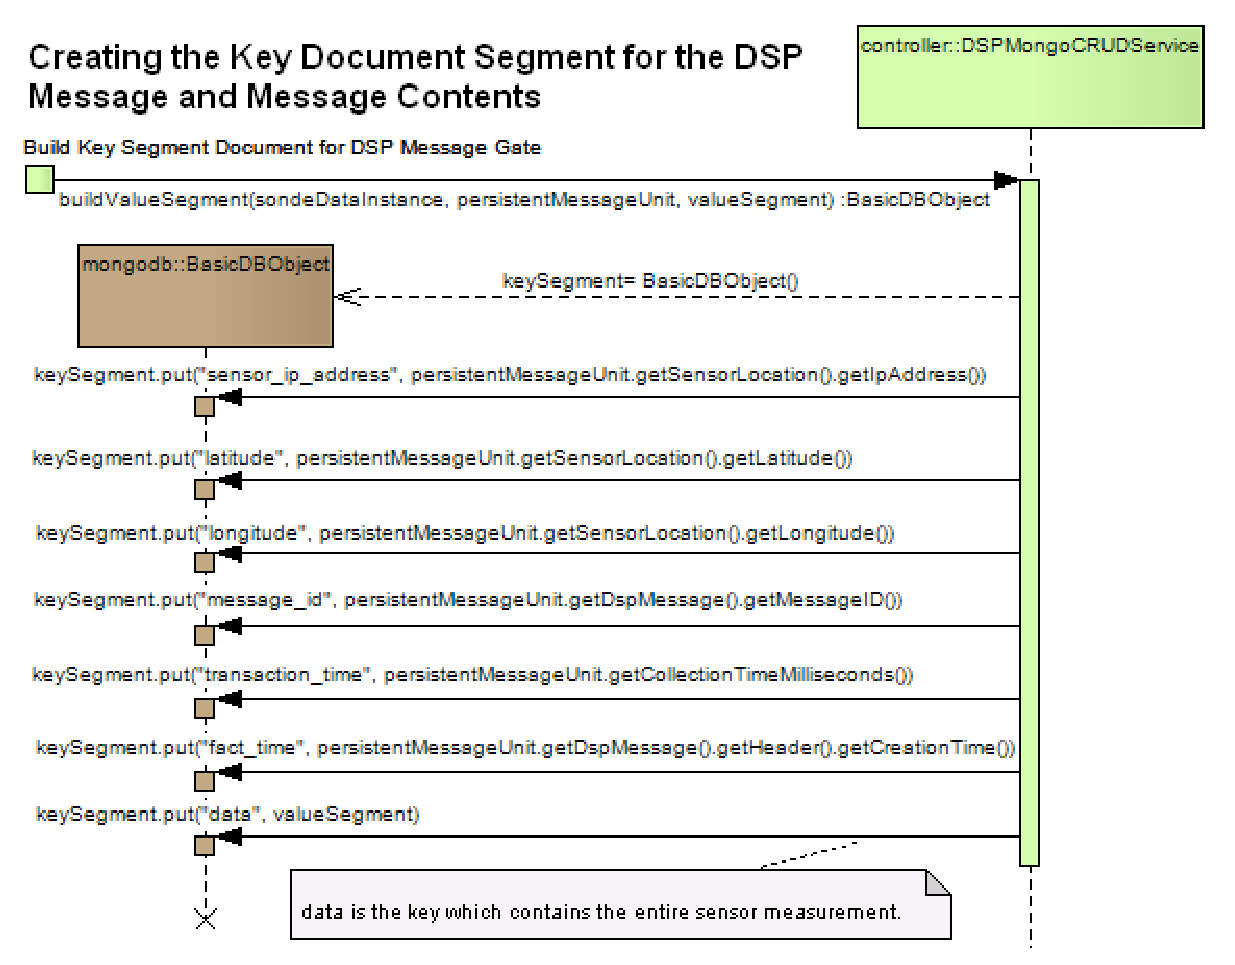
\includegraphics[scale=0.5]{../diagrams/From-Creating-Key-Segment-Sequence}
  \caption{UML Sequence diagram showing the creation of the key document segment}
  \label{fig:From-Creating-Key-Segment-Sequence}
\end{figure}

\section{DSP Data Persistence Deployment}

The deployment of the persistence layer is comprised by the addition of two
new components to the DSP Platform: the DSP Data Persistence and the MongoDB
Database Server. The former is responsible for capturing any data
produced by sensors in the data sink, as described in the previous sections of
this chapter. On the other hand, the latter is where the data is going to be
stored, as a result of the technology selection on the previous chapter. 

The deployment of the DSP Data Persistence follows the specifications of how to
deploy a DSP Component on an OSGi Framework. For the development of this work,
the Knopflerfish OSGi Container was used, as described in section
\ref{sec:dsp-data-persistence-implementation}. In contrast, the
deployment of the mongoDB can be accomplished in different approaches, as
summarized: 

\begin{itemize}
  \item \textbf{Single Server}: a regular deployment of a database system as it
  is done in general applications, where data is managed by one single process;
  \item \textbf{Sharded Server}: a deployment approach where data is sharded
  into different servers.
\end{itemize} 

The single server approach maintains all data located in a simple space.
Distributed Systems applications such as Master-Slave, Data Replication, etc
can be used in this approach for scalability
\ref{fig:DSP-Data-Persistence-Deployment-Single}. 

\begin{figure}[!b]
  \centering
  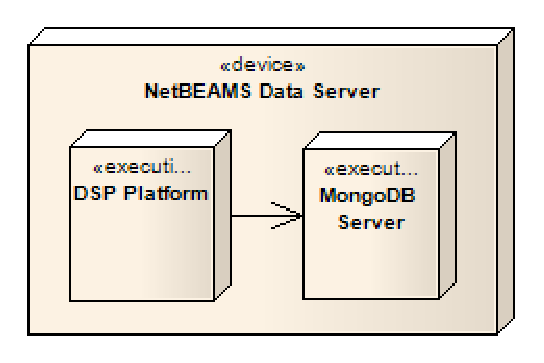
\includegraphics[scale=0.7]{../diagrams/DSP-Data-Persistence-Deployment-Single}
  \caption{UML Deployment diagram with a single server}
  \label{fig:DSP-Data-Persistence-Deployment-Single}
\end{figure}

However, given that mongoDB provides support to Shards, then the implementation
of a Data-Centric approach can be done by deploying different mongoDB instances
in a distributed cluster, where each node can hold a given type of data. The
specification of what types of data should be stored in each of the cluster
nodes is defined by a shard-key.

\begin{figure}[!b]
  \centering
  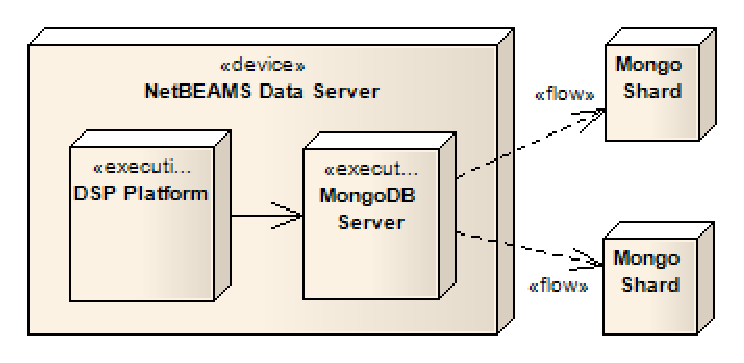
\includegraphics[scale=0.7]{../diagrams/DSP-Data-Persistence-Deployment-Sharded}
  \caption{UML Deployment Diagram for a sharded server}
  \label{fig:DSP-Data-Persistence-Deployment-Sharded}
\end{figure}

More details about the implementation of the DSP Data Persistence can be see in
the next chapter.